\documentclass[12pt,a4paper]{report}
\usepackage[utf8]{inputenc}
\usepackage[T1]{fontenc}
\usepackage{amsmath}
\usepackage{amsfonts}
\usepackage{amssymb}
\usepackage[urlbordercolor={0 0 1}]{hyperref}
\usepackage[left=2cm,right=2cm,top=2cm,bottom=2cm]{geometry}
\usepackage{graphicx} 
\usepackage{array}
 
\usepackage[francais]{babel}

\makeatletter
\def\maketitle{
  \null
  \begin{flushleft}
   
\includegraphics[width=6cm]{telecom_nancy.png}
  \end{flushleft}
  \vfill
  \begin{center}\leavevmode
    \normalfont
    {\LARGE \@title\par}
    {\Large \@date\par} 
    \vskip 1cm
    
  \end{center}
  \vfill
  \hfill
  \begin{flushright}
    {\Large \@author\par}
  \end{flushright}
  \cleardoublepage
  }
\makeatother
\date{2012-2013}
\author{Manon Signoret G32\\Thibaut Smith G32}
\title{Projet CSH\\Visualisation d'un r\'{e}seau de transport}

\renewcommand*\thesection{\arabic{section}} % jolies Sections

\begin{document}

\thispagestyle{empty}
\maketitle
\pagebreak

\section{Introduction}
Nous avons choisi le sujet 4, un programme permettant de visualiser un r\'{e}seau de transport. Le programme permet de d\'{e}finir et visualiser un r\'{e}seau de transport d'un type de marchandise : on peut d\'{e}finir l'espace g\'{e}ographique de travail de mani\`{e}re al\'{e}atoire (pour les tests), ou manuellement (avec un fichier .txt déjà existant ou avec une saisie manuelle sur la console). De plus, on peut aussi g\'{e}n\'{e}rer des chemins entre plusieurs d\'{e}pôts dans un ordre choisi. Le programme est \'{e}crit en C, et fonctionne enti\`{e}rement en ligne de commande. Le code est disponible sur \href{https://github.com/Videl/Graph-Visualization-Manager}{GitHub}.


\section{Cahier des charges}
Le programme avait plusieurs objectifs \`{a} r\'{e}aliser. En voici la liste, avec les solutions choisies pour atteindre l'objectif.

\begin{center}
  \begin{tabular}{|m{7cm}|m{7cm}|}
    \hline
    \textbf{Objectifs} & \textbf{Solutions} \\
    \hline
    Repr\'{e}sentation des graphes dans la m\'{e}moire       & Structures personnelles \\
    \hline
    Saisie d'informations venant de l'utilisateur    & Entr\'{e}es (\textbf{scanf}) \\
    \hline
    Repr\'{e}sentation des d\'{e}pôts                        & Structure et listes cha\^in\'{e}es simple \\
    \hline
    Algorithme de calcul du chemin optimum           & \href{https://en.wikipedia.org/wiki/Travelling_salesman_problem}{Travelling salesman problem}, Dijkstra \\
    \hline
    Possibilit\'{e} de d\'{e}finir le r\'{e}seau (nombre de d\'{e}p\^ots, leur localisation, les liaisons existantes)			     &	IHM \\
    \hline
    Choix du d\'{e}p\^ot source/destination(s)			 & IHM \\
    \hline
    Co\^ut de chaque liaison						 & IHM \\
    \hline
  	Visualisation du r\'{e}seau							 & Graphviz \\
    \hline
    Transformation fichier texte vers dot (Graphviz)     & Programme en C \\
    \hline
    Interface Homme-Machine (IHM)                    & Terminal (max 80 colonnes) \\
    \hline
    
  \end{tabular}
\end{center}

\section{Choix de conceptions}
Dans notre logiciel, une seule structure de données a été utilisée, nous avons donc choisi de ne créer que la structure dépôt, qui est caractérisée par son nom, sa distance avec le dépôt précédent et le sous-ensemble de dépôts suivants. En effet, au début du projet nous avions réfléchis sur le nombre de structures à créer en pensant également à une structure liaison qui pourrait symboliser les arcs entre les différents sommets (dépôts), puis nous avons choisi de ne pas la faire car après avoir commencé à coder, nous nous sommes rendus compte qu'elle était inutile. Ainsi voici, ci-dessous, une capture d'écran montrant la structure utilisée dans notre logiciel.

\begin{center}
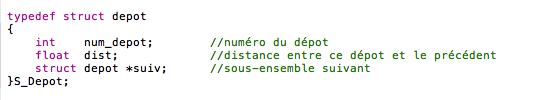
\includegraphics[scale=0.7]{capture2.png}
\end{center} 

\paragraph{Problème majeur survenu}
Tout d'abord, nous avons eu du mal \`{a} comprendre la documentation, et nous n'\'{e}tions pas s\^ur encore de quoi faire, et comment. Ce qui a retard\'{e} le projet. Nous sommes donc all\'{e}s chercher de l'aide d'abord vers un binôme en particulier\footnote{Clémence Henry, Pierre Monnin}, et ensuite sur Internet. Cela nous a d\'{e}bloqu\'{e}, et \`{a} partir de ce moment, le projet a pu commencer.
Pour expliquer comment fonctionne notre logiciel nous avons réalisé un bref schéma, ci-dessous.
\begin{center}
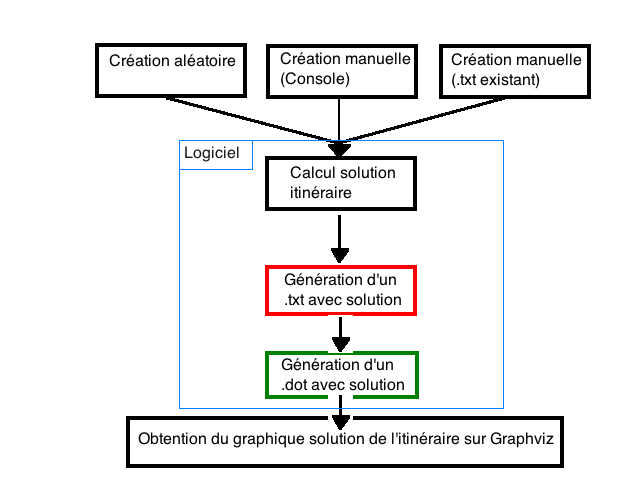
\includegraphics[scale=0.6]{conception.png}
\end{center} 
\paragraph{Calcul de l'itinéraire le plus court entre deux dépôts}
Cette partie là du logiciel a été assez longue. Nous avons donc créer une structure dépôt, et c'est dans cet ensemble là que le traitement des données se fait. Grâce à l'algorithme de Dijkstra (qui n'a pas posé de difficultés particulières), nous calculons le chemin le plus court entre le dépôt choisi en départ et celui en arrivée. Un problème survenu était que Manon Signoret travaille sur Mac et Thibaut Smith sur FreeBSD : l'encodage des fichiers textes contenant les informations était différents. Sous Mac, le programme se lançait mais indiquait une erreur, tandis que sur FreeBSD le programme fonctionnait comme prévu. (Ci-dessous une capture d'écran montrant le problème sous Mac.)
\begin{center}
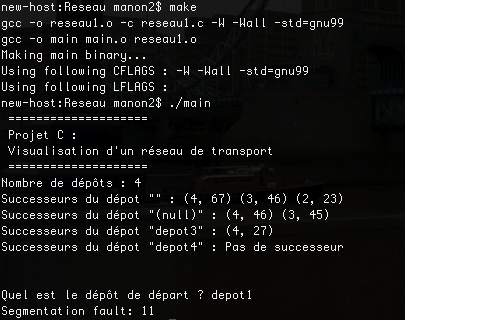
\includegraphics[scale=0.6]{capture1.png}
\end{center}
Pour subvenir à ce problème Manon Signoret, a donc travaillé sur Ubuntu (en double boot).

\paragraph{Génération d'un .txt avec la solution}
Avec la partie décrite ci-dessus nous obtenions donc le chemin optimal entre deux dépôts. Mais il a fallu générer cette solution sur un fichier .txt pour qu'il puisse être (dans l'étape suivante) transformé en un fichier \textit{.dot} compatible avec \textbf{Graphviz}. La solution se rajoute donc à la fin du fichier .txt contenant les données, grâce a la commande \textit{$fseek(Fichier, 0, SEEK\_END);$} qui nous permet de se place à la fin d'un fichier. METTRE UNE PHOTO DU .TXT QUI MONTRE LA FIN AVEC LE NOM DES DEPOTS QUI S'AJOUTENT. L'un des problèmes redondants était qu'il fallait souvent réajuster le script qui transformait le fichier texte en fichier dot compatible avec Graphviz : au fur et à mesure que l'on rajoutait des informations dans le fichier texte, il fallait le prendre en compte dans le programme de traduction \textit{.txt > .dot}.

\paragraph{Génération d'un .dot avec la solution}
Après l'étape précédente, le plus important était de connaître comment fonctionnait Graphviz pour générer un fichier .dot lisible par ce logiciel. Ainsi nous avons regardé la documentation sur internet et nous avons pu nous inspirer d'une structure générale, ci-dessous.
\begin{center}
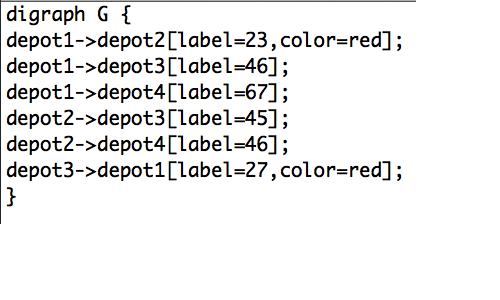
\includegraphics[scale=0.4]{capture3.png}
\end{center}
DIRE LES PROBLEMES QUE TU AS RENCONTRES

\section{Représentation visuelle du logiciel}
Voici quelques captures d'écran montrant ce que notre logiciel fait sur la console. (EN METTRE TROIS ENVIRON ET UNE LIGNE DE DESCRIPTION)

\paragraph{Graphviz}
Voilà maintenant ce que nous obtenons grâce aux .dot générés par notre logiciel, grâce au logiciel Graphviz. Nous avons coloré en rouge le chemin optimal de l'itinéraire en solution.

\begin{center}
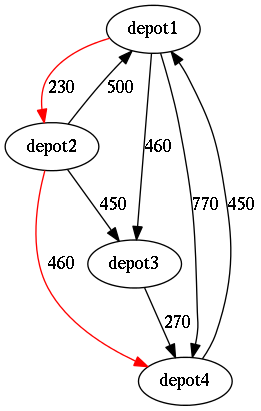
\includegraphics[scale=0.6]{output.png}
\end{center}

Le programme de traduction \textit{.txt > .dot} peut se découper en partie :


\begin{enumerate}
\item lecture du fichier de données et demande de mémoire à l'OS 
\item capture des informations et sauvegarde dans des tableaux/variables 
\item sauvegarde de ces informations dans un fichier de sortie, dans un format compréhensible par \textbf{Graphviz}
\item libération de la mémoire. 
\end{enumerate}

Des problèmes et des bugs sont apparus dans chaque parties de ce programme. Nous avons corriger le plus possible de bug grâce aux outils \textbf{gdb} et \textbf{valgrind} ainsi que les paramètres de compilation $-W -Wall -std=gnu99$, qui se sont avérés très utiles.

\section{Gestion du code source}
Nous avons choisi d'utiliser Git pour ce projet, \'{e}tant donn\'{e} que nous avions d\'{e}j\`{a} utilis\'{e} SVN\footnote{Il ne manque plus que Bazaar, Mercurial, etc!}. La forge de l'\'{e}cole ne supportant pas Git, nous avons choisi d'h\'{e}berger notre code source sur \href{https://github.com/Videl/Graph-Visualization-Manager}{GitHub}. C'était une première pour Manon Signoret qui ne le connaissait pas encore. Il s'est avéré qu'il est très facile d'utilisation et très pratique, plus que SVN à notre goût.

\section{Nombre d'heures}
Nous avons pass\'{e} un nombre important d'heures sur la compr\'{e}hension de la documentation de Graphviz avant de savoir quoi faire, Graphviz fonctionnant avec ses propres structures.

\begin{tabular}{|c|c|}
  \hline
  Travail & Heures \\
  \hline
  Doc' Graphviz & ~5H \\
  \hline
  D\'{e}veloppement	&	~10H \\
  \hline
  Tests	&	~5H \\ 
  \hline
  Rapport	&	~3H \\
  \hline
\end{tabular}

\section{Sources}

\end{document}
